\documentclass[journal,12pt,twocolumn]{IEEEtran}
%
\usepackage{setspace}
\usepackage{gensymb}
%\doublespacing
\singlespacing

%\usepackage{graphicx}
%\usepackage{amssymb}
%\usepackage{relsize}
\usepackage[cmex10]{amsmath}
%\usepackage{amsthm}
%\interdisplaylinepenalty=2500
%\savesymbol{iint}
%\usepackage{txfonts}
%\restoresymbol{TXF}{iint}
%\usepackage{wasysym}
\usepackage{amsthm}
\usepackage{mathrsfs}
\usepackage{txfonts}
\usepackage{stfloats}
\usepackage{steinmetz}
\usepackage{bm}
\usepackage{cite}
\usepackage{cases}
\usepackage{subfig}
%\usepackage{xtab}
\usepackage{longtable}
\usepackage{multirow}
%\usepackage{algorithm}
%\usepackage{algpseudocode}
\usepackage{enumitem}
\usepackage{mathtools}
\usepackage{tikz}
\usepackage{circuitikz}
\usepackage{verbatim}
\usepackage{tfrupee}
\usepackage[breaklinks=true]{hyperref}
%\usepackage{stmaryrd}
\usepackage{tkz-euclide} % loads  TikZ and tkz-base
%\usetkzobj{all}
\usepackage{listings}
    \usepackage{color}                                            %%
    \usepackage{array}                                            %%
    \usepackage{longtable}                                        %%
    \usepackage{calc}                                             %%
    \usepackage{multirow}                                         %%
    \usepackage{hhline}                                           %%
    \usepackage{ifthen}                                           %%
  %optionally (for landscape tables embedded in another document): %%
    \usepackage{lscape}     
\usepackage{multicol}
\usepackage{chngcntr}
%\usepackage{enumerate}

%\usepackage{wasysym}
%\newcounter{MYtempeqncnt}
\DeclareMathOperator*{\Res}{Res}
%\renewcommand{\baselinestretch}{2}
\renewcommand\thesection{\arabic{section}}
\renewcommand\thesubsection{\thesection.\arabic{subsection}}
\renewcommand\thesubsubsection{\thesubsection.\arabic{subsubsection}}

\renewcommand\thesectiondis{\arabic{section}}
\renewcommand\thesubsectiondis{\thesectiondis.\arabic{subsection}}
\renewcommand\thesubsubsectiondis{\thesubsectiondis.\arabic{subsubsection}}

% correct bad hyphenation here
\hyphenation{op-tical net-works semi-conduc-tor}
\def\inputGnumericTable{}                                 %%

\lstset{
%language=C,
frame=single, 
breaklines=true,
columns=fullflexible
}
%\lstset{
%language=tex,
%frame=single, 
%breaklines=true
%}

\begin{document}
%


\newtheorem{theorem}{Theorem}[section]
\newtheorem{problem}{Problem}
\newtheorem{proposition}{Proposition}[section]
\newtheorem{lemma}{Lemma}[section]
\newtheorem{corollary}[theorem]{Corollary}
\newtheorem{example}{Example}[section]
\newtheorem{definition}[problem]{Definition}
%\newtheorem{thm}{Theorem}[section] 
%\newtheorem{defn}[thm]{Definition}
%\newtheorem{algorithm}{Algorithm}[section]
%\newtheorem{cor}{Corollary}
\newcommand{\BEQA}{\begin{eqnarray}}
\newcommand{\EEQA}{\end{eqnarray}}
\newcommand{\define}{\stackrel{\triangle}{=}}
\bibliographystyle{IEEEtran}
%\bibliographystyle{ieeetr}
\providecommand{\mbf}{\mathbf}
\providecommand{\pr}[1]{\ensuremath{\Pr\left(#1\right)}}
\providecommand{\qfunc}[1]{\ensuremath{Q\left(#1\right)}}
\providecommand{\sbrak}[1]{\ensuremath{{}\left[#1\right]}}
\providecommand{\lsbrak}[1]{\ensuremath{{}\left[#1\right.}}
\providecommand{\rsbrak}[1]{\ensuremath{{}\left.#1\right]}}
\providecommand{\brak}[1]{\ensuremath{\left(#1\right)}}
\providecommand{\lbrak}[1]{\ensuremath{\left(#1\right.}}
\providecommand{\rbrak}[1]{\ensuremath{\left.#1\right)}}
\providecommand{\cbrak}[1]{\ensuremath{\left\{#1\right\}}}
\providecommand{\lcbrak}[1]{\ensuremath{\left\{#1\right.}}
\providecommand{\rcbrak}[1]{\ensuremath{\left.#1\right\}}}
\theoremstyle{remark}
\newtheorem{rem}{Remark}
\newcommand{\sgn}{\mathop{\mathrm{sgn}}}
\providecommand{\abs}[1]{\left\vert#1\right\vert}
\providecommand{\res}[1]{\Res\displaylimits_{#1}} 
\providecommand{\norm}[1]{\left\lVert#1\right\rVert}
%\providecommand{\norm}[1]{\lVert#1\rVert}
\providecommand{\mtx}[1]{\mathbf{#1}}
\providecommand{\mean}[1]{E\left[ #1 \right]}
\providecommand{\fourier}{\overset{\mathcal{F}}{ \rightleftharpoons}}
%\providecommand{\hilbert}{\overset{\mathcal{H}}{ \rightleftharpoons}}
\providecommand{\system}{\overset{\mathcal{H}}{ \longleftrightarrow}}
	%\newcommand{\solution}[2]{\textbf{Solution:}{#1}}
\newcommand{\solution}{\noindent \textbf{Solution: }}
\newcommand{\cosec}{\,\text{cosec}\,}
\providecommand{\dec}[2]{\ensuremath{\overset{#1}{\underset{#2}{\gtrless}}}}
\newcommand{\myvec}[1]{\ensuremath{\begin{pmatrix}#1\end{pmatrix}}}
\newcommand{\mydet}[1]{\ensuremath{\begin{vmatrix}#1\end{vmatrix}}}
%\numberwithin{equation}{section}
\numberwithin{equation}{subsection}
%\numberwithin{problem}{section}
%\numberwithin{definition}{section}
\makeatletter
\@addtoreset{figure}{problem}
\makeatother
\let\StandardTheFigure\thefigure
\let\vec\mathbf
%\renewcommand{\thefigure}{\theproblem.\arabic{figure}}
\renewcommand{\thefigure}{\theproblem}
%\setlist[enumerate,1]{before=\renewcommand\theequation{\theenumi.\arabic{equation}}
%\counterwithin{equation}{enumi}
%\renewcommand{\theequation}{\arabic{subsection}.\arabic{equation}}
\def\putbox#1#2#3{\makebox[0in][l]{\makebox[#1][l]{}\raisebox{\baselineskip}[0in][0in]{\raisebox{#2}[0in][0in]{#3}}}}
     \def\rightbox#1{\makebox[0in][r]{#1}}
     \def\centbox#1{\makebox[0in]{#1}}
     \def\topbox#1{\raisebox{-\baselineskip}[0in][0in]{#1}}
     \def\midbox#1{\raisebox{-0.5\baselineskip}[0in][0in]{#1}}
\vspace{3cm}
\title{
SM5083 - BASICS OF PROGRAMMING
	}
\author{ RS Girish - EE20RESCH14005$^{*}$% <-this % stops a space
\thanks{*The author is with the Department
		of Electrical Engineering, Indian Institute of Technology, Hyderabad
		502285 India e-mail:  ee20resch14005@iith.ac.in. All content in this document is released under GNU GPL.  Free and open source.}
	}
\maketitle
\newpage
\tableofcontents
\bigskip
\renewcommand{\thefigure}{\theenumi}
\renewcommand{\thetable}{\theenumi}
\begin{abstract}
This paper contains solution to problem no 5 of Examples III Section of Chapter III of Analytical Geometry by Hukum Chand.
Links to Python codes are available below.  
\end{abstract}
Download python codes at 
\begin{lstlisting}
https://github.com/rsgirishkumar/SM5083/ASSIGNMENT2
\end{lstlisting}
\section{Problem}
The opposite vertices of a square are $\myvec{0\\-1},\myvec{0\\3}$. Find the equations of four sides.
\section{Solution}
Let the given points are indicated as below\\
\begin{align}
\begin{split}
\vec{A} = \myvec{0 \\ -1}, 
\vec{C} = \myvec{0 \\ 3}.\\
\end{split}
\end{align}
Let the unknown vertices are indicated as $ \vec{B},\vec{D}$. The step by step procedure involves
\begin{enumerate}
	\item By doing affine transformation steps i.e Translation and Rotation of the given vertices $\vec{A}$ and $\vec{C}$ to origin, those provide $\vec{A^{'}}$ and $\vec{C^{'}}$ for the ease of solution 
    \item Find the diagonal/Direction vector $\vec{AC}$.
    \item Find the norm of $\vec{AC}$.
    \item Find the points $\vec{B}$ and $\vec{D}$ by using inspection method and reverse affine transformation.
    \item Form the equations of lines using vertices.
\end{enumerate}
\subsection{USING AFFINE TRANSFORMATION}
\textbf{Translation and Rotation}
Lets consider a square with origin($\vec{O}$) as a vertex and x, y - axes are two sides.  Let the other vertices be $\vec{F,G,H}$. For the Square that has to be formed with the vertices given be denoted by $\vec{ABCD}$. To obtain $\vec{ABCD}$ from $\vec{OFGH}$ or viceversa, Affine transformation has to be applied.This eases out the process of finding the vertices.
\\
Let $\vec{P}$ be translation vector is given by $\vec{P} = \vec{O}-\vec{A}$, and the angle to be rotated be $\theta$ for $\vec{AC}$ to align with $\vec{OG}$, then the angle $\theta$ and rotation matrix $\vec{R}$ is given by
\begin{align}
\begin{split}
cos(\theta) = \frac{(\vec{C}-\vec{A})^T.1}{||(\vec{C}-\vec{A})^T||}\\
\vec{R}=\myvec{cos(\theta) & -sin(\theta)\\sin(\theta) & cos(\theta)}\\ 
\end{split}
\end{align}
\\
The points can be obtained by using the generalized affine transformation principle as below
\begin{align}
\begin{split}
\vec{A^{'}} = \vec{R}(\vec{A+P})\\
\vec{C^{'}} = \vec{R}(\vec{C+P})\\
\end{split}
\end{align}
\\
In general $\vec{A^{'}} = \vec{O}$.
\\
The length of $\vec{A^{'}B^{'}}$ based on projection on to $\vec{A^{'}C^{'}}$ and the projection of $\vec{A^{'}C^{'}}$ on to $\vec{A^{'}B^{'}}$ is given by \\
\begin{align}
\begin{split}
||\vec{A^{'}B^{'}}|| = \frac{||\vec{A^{'}C^{'}}||}{cos(\theta)}\\
\vec{A^{'}B^{'}} = ||\vec{A^{'}B^{'}}||\vec{OF}\\
\vec{B^{'}}=\vec{A^{'}B^{'}}+\vec{A^{'}}\\
\end{split}
\end{align}
In the similar way, 
\begin{align}
\begin{split}
||\vec{A^{'}D^{'}}|| = \frac{||\vec{A^{'}C^{'}}||}{cos(\theta)}\\
\vec{A^{'}D^{'}} = ||\vec{A^{'}D^{'}}||\vec{OH}\\
\vec{D^{'}}=\vec{A^{'}D^{'}}+\vec{A^{'}}\\
\end{split}
\end{align}
By doing the reverse affine transformation, the Square $\vec{ABCD}$ can be obtained from $\vec{A^{'}B^{'}C^{'}D^{'}}$ by using the below transformation principles.\\
\begin{align}
\begin{split}
\vec{A} = \vec{R^{-1}A^{'}}-\vec{P}\\
\vec{B} = \vec{R^{-1}B^{'}}-\vec{P}\\
\vec{C} = \vec{R^{-1}C^{'}}-\vec{P}\\
\vec{D} = \vec{R^{-1}D^{'}}-\vec{P}\\
where\\
\vec{R^{-1}} = \myvec{cos(-\theta)& -sin(-\theta)\\sin(-\theta)&cos(-\theta)} \ and\\
\vec{P} = \vec{O} - \vec{A}.
\end{split}
\end{align}
\bigskip
\begin{figure}
	\centering
    \resizebox{\columnwidth}{!}{
	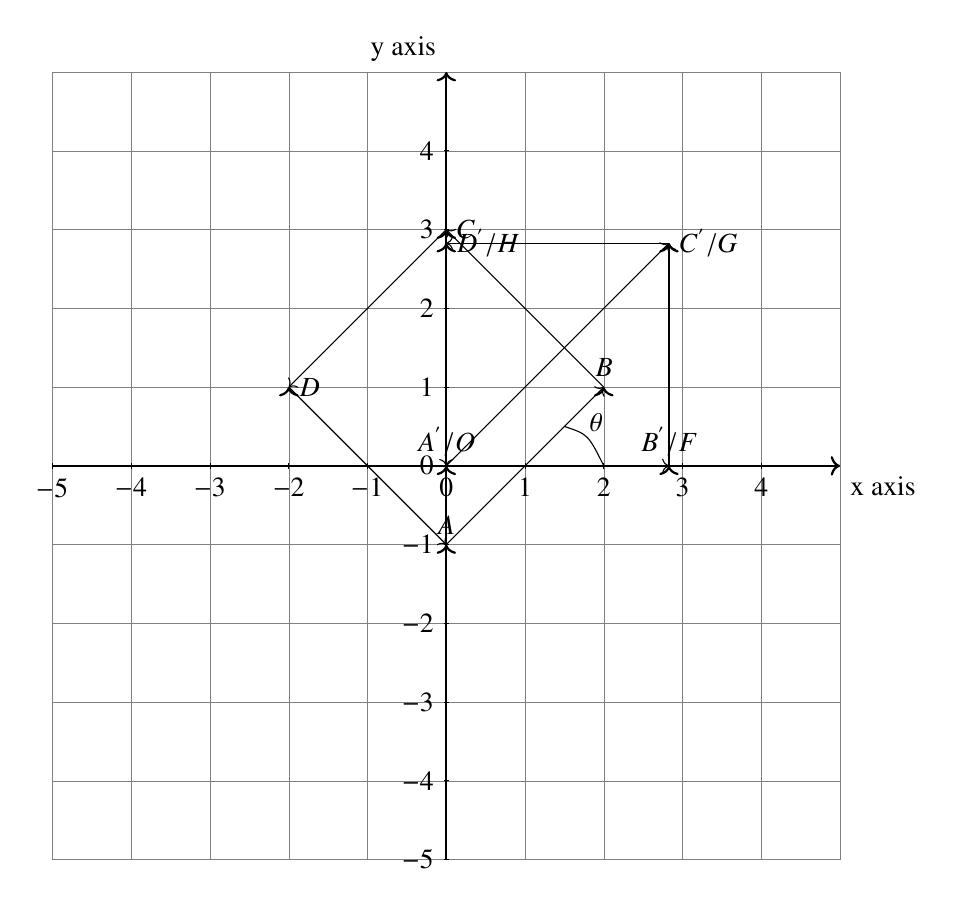
\begin{tikzpicture}
		\draw[step=1cm,gray,very thin] (-5,-5) grid (5,5);
		\draw[thick,->] (-5,0) -- (5,0) node[anchor=north west] {x axis};
		\draw[thick,->] (0,-5) -- (0,5) node[anchor=south east] {y axis};
		\foreach \x in {-5,-4,-3,-2,-1,0,1,2,3,4}
   			\draw (\x cm,1pt) -- (\x cm,-1pt) node[anchor=north] {$\x$};
		\foreach \y in {-5,-4,-3,-2,-1,0,1,2,3,4}
    		\draw (1pt,\y cm) -- (-1pt,\y cm) node[anchor=east] {$\y$};
		\draw [->] (0,-1) -- (2,1);
		\draw [->] (2,1) -- (0,3);
		\draw [->] (0,3) -- (-2,1);
		\draw [->] (-2,1) -- (0,-1);
		\draw [thick, ->] (0,-1) node[anchor=south] {$A$};
		\draw [thick, ->] (2,1) node[anchor=south] {$B$};
		\draw [thick, ->] (0,3) node[anchor=west] {$C$};
		\draw [thick, ->] (-2,1) node[anchor=west] {$D$};
		\draw [->] (0,0) -- (2.828,0);
		\draw [->] (2.828,0) -- (2.828,2.828);
		\draw [->] (2.828,2.828) -- (0,2.828);
		\draw [->] (0,2.828) -- (0,0);
		\draw [->] (0,0) -- (2.828,2.828);
		\draw [thick, ->] (0,0) node[anchor=south] {$A^{'}/O$};
		\draw [thick, ->] (2.828,0) node[anchor=south] {$B^{'}/F$};
		\draw [thick, ->] (2.828,2.828) node[anchor=west] {$C^{'}/G$};
		\draw [thick, ->] (0,2.828) node[anchor=west] {$D^{'}/H$};
		\draw (1.5,0.5) .. controls (1.8,0.4)..(2,0);
		\draw [thick] (1.9,0.3) node[anchor=south] {$\theta$};
		\end{tikzpicture}
	}
	\caption{SQUARE ABCD and OFGH/A'B'C'D'}
    \label{fig:SQUARE ABCD and OFGH/A'B'C'D'}
\end{figure}
\\
Diagonal(Direction Vector) $\vec{AC} = \vec{C}-\vec{A} $  is given by
\begin{align}
\begin{split}
\vec{AC} = \myvec{0 - 0\\3 - (-1)} = \myvec{0\\4}.\\
\end{split}
\end{align}
\\
Translation for $\vec{A}$ to $\vec{O}$ requries a translation vector $ \vec{P}=\myvec{0\\1}$.
\begin{align}
\begin{split}
\Rightarrow
\vec{A^{'}} = \myvec{0 \\ -1}  + \myvec{0\\1} = \myvec{0\\0} &\\
\vec{C^{'}} = \myvec{0 \\ 3} + \myvec{0\\1} = \myvec{0\\4}.\\
\vec{A^{'}C^{'}} = \myvec{0 - 0\\4- 0} = \myvec{0\\4}.\\
\end{split}
\end{align}
\\
Norm of $\vec{A^{'}C^{'}}$
\begin{align}
\begin{split}
\Vert\vec{A^{'}C^{'}}\Vert = \sqrt{(2\sqrt{2})^{2}+(2\sqrt{2})^{2}} = 4
\end{split}
\end{align}
\\
The rotation is by $45^{o}$ clock wise. The rotation matrix is given by 
\begin{align}
\begin{split}
\myvec{cos(-45^{o}) & -sin(-45^{o})\\sin(-45^{o}) & cos(-45^{o})}\\ 
\Rightarrow \vec{A^{'}C^{'}} =   \myvec{\frac{1}{\sqrt{2}} & \frac{1}{\sqrt{2}} \\ -\frac{1}{\sqrt{2}} & \frac{1}{\sqrt{2}}} \myvec{0 \\ 4}= \myvec{2\sqrt{2}\\2\sqrt{2}}\\
\vec{C^{'}}=\vec{A^{'}C^{'}}+\vec{A^{'}}=\myvec{2\sqrt{2}\\2\sqrt{2}}\\
\end{split}
\end{align}
\\
The line equation of $\vec{A^{'}C^{'}}$ is x-y=0 or simply x=y.\\
By inspection method,
using length of a side, the vertices $\vec{B^{'}}$ and $\vec{D^{'}}$ can be found.\\
\begin{align}
\begin{split}
\Vert\vec{A^{'}B^{'}}\Vert = \frac{\Vert\vec{A^{'}C^{'}}\Vert}{\sqrt{2}} = \frac{4}{\sqrt{2}}=2\sqrt{2}.\\
Also, \vec{OF} = \myvec{1\\0}\\
\vec{A^{'}B^{'}} = \Vert\vec{A^{'}B^{'}}\Vert\vec{OF}=2\sqrt{2}*\myvec{1\\0}=\myvec{2\sqrt{2}\\0}.\\
\vec{B^{'}} = \vec{A^{'}B^{'}}+\vec{A^{'}}=\myvec{2\sqrt{2}\\0}\\
\end{split}
\end{align}
\begin{align}
\begin{split}
\Vert\vec{A^{'}D^{'}}\Vert = \frac{\Vert\vec{A^{'}C^{'}}\Vert}{\sqrt{2}} = \frac{4}{\sqrt{2}}=2\sqrt{2}.\\
Also, \vec{OH} = \myvec{0\\1}\\
\vec{A^{'}D^{'}} = \Vert\vec{A^{'}D^{'}}\Vert\vec{OH}=2\sqrt{2}*\myvec{0\\1}=\myvec{0\\2\sqrt{2}}.\\
\vec{D^{'}} = \vec{A^{'}D^{'}}+\vec{A^{'}}=\myvec{0\\2\sqrt{2}}\\
\end{split}
\end{align}
\\
Hence the obtained vertices are 
\begin{align}
\begin{split}
\vec{A^{'}} = \myvec{0 \\ 0},
\vec{B^{'}} = \myvec{2\sqrt{2}\\0}
\vec{C^{'}} = \myvec{2\sqrt{2}\\2\sqrt{2}}.
\vec{D^{'}} = \myvec{0\\2\sqrt{2}}.
\end{split}
\end{align}
\subsection{USING REVERSE AFFINE TRANSFORMATION}
The rotation is by $45^{o}$ counter clock wise i.e. $\theta = 45^{o}$. The inverse of rotation matrix $\vec{R}$ is given by 
\begin{align}
\begin{split}
\vec{R^{-1}} = \frac{1}{1}\myvec{\frac{1}{\sqrt{2}}&-\frac{1}{\sqrt{2}}\\\frac{1}{\sqrt{2}}&\frac{1}{\sqrt{2}}}\\
\end{split}
\end{align} and the translation vector is $\vec{-P}$.
From above reverse affine transformation principles,
\begin{align}
\begin{split}
\vec{A} = \myvec{\frac{1}{\sqrt{2}}&-\frac{1}{\sqrt{2}}\\\frac{1}{\sqrt{2}}&\frac{1}{\sqrt{2}}}\myvec{0 \\ 0}  + \myvec{0\\-1} = \myvec{0\\-1}\\
\vec{B} = \myvec{\frac{1}{\sqrt{2}}&-\frac{1}{\sqrt{2}}\\\frac{1}{\sqrt{2}}&\frac{1}{\sqrt{2}}}\myvec{2\sqrt{2} \\ 0}  + \myvec{0\\-1} = \myvec{2\\1}\\
\vec{C} = \myvec{\frac{1}{\sqrt{2}}&-\frac{1}{\sqrt{2}}\\\frac{1}{\sqrt{2}}&\frac{1}{\sqrt{2}}}\myvec{2\sqrt{2} \\ 2\sqrt{2}} + \myvec{0\\-1} = \myvec{0\\3}.\\
\vec{D} = \myvec{\frac{1}{\sqrt{2}}&-\frac{1}{\sqrt{2}}\\\frac{1}{\sqrt{2}}&\frac{1}{\sqrt{2}}}\myvec{0 \\ 2\sqrt{2}}  + \myvec{0\\-1} = \myvec{-2\\1}\\
\end{split}
\end{align}
\subsection{LINE EQUATIONS}
Coordinates are
\\
\begin{align}
\begin{split}
\vec{A} = \myvec{0 \\ -1},
\vec{B} =\myvec{-2\\1} ,
\vec{C} = \myvec{0 \\ 3},
\vec{D} =\myvec{2\\1}.
\end{split}
\end{align}
In Matrix form, if $\myvec{X_1\\Y_1} \&  \myvec{X_2\\Y_2}$ are the points given then the directional vector is given by \\$\myvec{X_2-X_1\\ Y_2-Y_1}$ \\then, 
the form of equation ax+by+c=0 can be written as\\ 
\begin{align}
\begin{split}
a= \vec{Y_2-Y_1},\\ b=-(\vec{X_2-X_1}),\\ c = \myvec{\vec{Y_2}&-\vec{X_2}} \myvec{\vec{X_2-X_1}\\\vec{ Y_2-Y_1}}
\end{split}
\end{align}
\\
\\
By using the same, the line equation $\vec{AB}$ for points $\vec{A} = \myvec{0\\-1},\vec{B}=\myvec{-2\\1}$ is as follows:
\\
\begin{align}
\begin{split}
\vec{AB} = \myvec{-2\\2}\\
a=2,\ b=2,\\
c=\myvec{-1 & 0} \myvec{-2\\2}=2\\
\end{split}
\end{align}
Line equation for $\vec{AB}$
\begin{align}
\begin{split}
\Rightarrow\ 2x+2y+2=0 \ or \ x+y=-1. \\
\end{split}
\end{align}
In vector form
\begin{align}
\begin{split}
\Rightarrow \myvec{1&1}\ \vec{X}=-1\\
\end{split}
\end{align}
\\
The line equation $\vec{BC}$ for points $\vec{B} = \myvec{-2\\1},\vec{C}=\myvec{0\\3}$ is as follows:
\\
\begin{align}
\begin{split}
\vec{BC} = \myvec{2\\2}\\
a=2,\ b=-2,\\
c=\myvec{1 & 2} \myvec{2\\2}=6\\
\end{split}
\end{align}
Line equation for $\vec{BC}$
\begin{align}
\begin{split}
\Rightarrow\ 2x-2y+6=0 \ or \ x-y=-3. \\
\end{split}
\end{align}
In vector form
\begin{align}
\begin{split}
\Rightarrow \myvec{1&-1}\ \vec{X}=-3
\end{split}
\end{align}
\\
The line equation $\vec{CD}$ for points $\vec{C}=\myvec{0\\3},\vec{D} = \myvec{2\\1}$ is as follows:
\\
\begin{align}
\begin{split}
\vec{CD} = \myvec{2\\-2}\\
a=-2,\ b=-2,\\
c=\myvec{3 & 0} \myvec{2\\-2}=6\\
\end{split}
\end{align}
Line equation for $\vec{CD}$
\begin{align}
\begin{split}
 \Rightarrow\ -2x-2y+6=0 \ or \ x+y=3. \\
\end{split}
\end{align}
In vector form
\begin{align}
\begin{split}
\Rightarrow \myvec{1&1}\ \vec{X}=3
\end{split}
\end{align}
\\
The line equation $\vec{DA}$ for points $\vec{D} = \myvec{2\\1}, \vec{A} = \myvec{0\\-1}$ is as follows:\\
\begin{align}
\begin{split}
\vec{DA} = \myvec{-2\\-2}\\
a=-2,\ b=2,\\
c=\myvec{1 & -2} \myvec{-2\\-2}=2\\
\end{split}
\end{align}
Line equation for $\vec{DA}$
\begin{align}
\begin{split}
\Rightarrow\ -2x+2y+2=0 \ or \ x-y=1. \\
\end{split}
\end{align}
In vector form
\begin{align}
\begin{split}
\Rightarrow \myvec{1&-1}\ \vec{X}=1
\end{split}
\end{align}.
\\
The plotted graph is shown as below.
\begin{figure}[!ht]
    \centering
    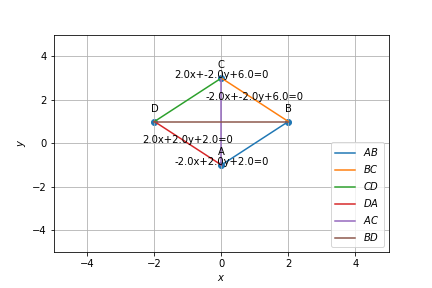
\includegraphics[width=\columnwidth]{assignment2_using affine.png}
    \caption{Square ABCD}
    \label{fig:Square ABCD}
\end{figure}
\end{document}